\documentclass{beamer}
\beamertemplatenavigationsymbolsempty
\usecolortheme{beaver}
\setbeamertemplate{blocks}[rounded=true, shadow=true]
\setbeamertemplate{footline}[page number]

\usepackage[utf8]{inputenc}
\usepackage[english,russian]{babel}
\usepackage{amssymb,amsfonts,amsmath,mathtext}
\usepackage{algorithm}
\usepackage{algpseudocode}
\makeatletter
\renewcommand{\ALG@name}{Алгоритм}
\makeatother

\newcommand{\dotprod}[2]{\left\langle #1,#2 \right\rangle}
\newcommand{\expect}[1]{\mathbb{E}\left[ #1 \right]}
\newcommand{\norms}[1]{\left\| #1 \right\|}

%----------------------------------------------------------------------------------------------------------

\title[\hbox to 56mm{Применение стохастической аппроксимации нулевого порядка с техникой запоминания в алгоритме Франка-Вульфа}]{Применение стохастической аппроксимации нулевого порядка с техникой запоминания в алгоритме Франка-Вульфа}
\author[А. Б. Богданов]{Александр Иванович Богданов \\
                        $ $ \\ 
                        Научный руководитель: \\
                        к.ф.-м.н. Безносиков А. Н.}
\institute[]{Московский физико-технический институт \\
             ФПМИ \\
             Кафедра <<Интеллектуальные системы>>}
\date{}

%----------------------------------------------------------------------------------------------------------

\begin{document}

%----------------------------------------------------------------------------------------------------------

\begin{frame}

    \maketitle

\end{frame}

%-----------------------------------------------------------------------------------------------------

\begin{frame}{Цель исследования}

    \textbf{Проблема:} Ставится выпуклая задача оптимизации на ограниченном выпуклом множестве с доступом только к зашумленному нулевому оракулу. \\

    $ $\\

    \textbf{Цель:} Предложить робастый алгоритм, аппроксимирующий градиент, использующий $\mathcal{O}(1)$ вызовов оракула на каждой итерации.\\

    $ $\\

    \textbf{Решение:} Предлагается модификация JAGUAR, которая использует технику запоминания.
    
\end{frame}

%-----------------------------------------------------------------------------------------------------

\begin{frame}{Литература}
    \begin{itemize}
        \item Marguerite Frank and Philip Wolfe. An algorithm for quadratic programming. Naval research logistics quarterly, 3(1-2):95–110, 1956.
        \item   
        \item
        \item 
    \end{itemize}

\end{frame}

%-----------------------------------------------------------------------------------------------------

\begin{frame}{Постановка задачи}

    Рассматривается две оптимизационные задачи:\\

    \begin{itemize}
        \item Нестохастическая
                
                \begin{equation*}
                    \underset{x \in Q}{\min} \quad f(x)
                \end{equation*}

            Доступ только к $f_{\delta}(x) := f(x) + \delta(x)$, где $\delta(x)$ - шум.

            $f(x)$ -- выпуклая на $Q$ функция.

        \item Стохастическая
        
                \begin{equation*}
                    \underset{x \in Q}{\min} \quad f(x) := 
                    \mathbb{E}_{\xi}\left[f(x, \xi)\right],
                \end{equation*}

                
            Доступ только к $f_{\delta}(x, \xi) := f(x, \xi) + \delta(x, \xi)$, где $\delta(x, \xi)$ - шум.

            $f(x, \xi)$ -- выпуклая на $Q$ функция.

    \end{itemize}

        $Q \subseteq \mathbb{R}^d$ - произвольное выпуклое ограниченное множество.
   
\end{frame}

%----------------------------------------------------------------------------------------------------------

% \begin{frame}{JAGUAR. Нестохастический случай}

%     Разностная схема, которая будет использоваться в алгоритме:

%         \begin{equation*}
%             \widetilde{\nabla}_if_\delta(x) :=  \dfrac{f_\delta(x + \gamma e_i) - f_\delta(x - \gamma e_i)}{2 \gamma} e_i,
%         \end{equation*}

%     где $e_i$ - $i$-ый базисный вектор, $\gamma$ - параметр сглаживания.

%     \begin{algorithm}[H]
%     	\caption{JAGUAR. Нестохастический случай}        	
%         \begin{algorithmic}[1]
%         	\State {\bf Вход:} $x, h \in \mathbb{R}^d$
          
%             \State Сэмплируем $i \in \overline{1, d}$ независимо и равномерно
    
%             \State Считаем $\widetilde{\nabla}_i f_{\delta}(x) = \dfrac{f_{\delta}(x + \gamma e_i) - f_{\delta}(x - \gamma e_i)}{2 \gamma} e_i$
    
%             \State $g = g - \dotprod{h}{e_i} e_i + \widetilde{\nabla}_i f_{\delta}(x)$
        
%             \State \textbf{Выход:} $g$ 
%             \end{algorithmic}
%     \end{algorithm}


% \end{frame}

%----------------------------------------------------------------------------------------------------------

\begin{frame}{Обычный Франк-Вульф}

    Общие допущения:
    \begin{enumerate}
        \item Ограниченность множества $Q$:
            \begin{equation*}
                \forall x, y \in Q \hookrightarrow \norms{x- y}^2 \leq  D^2.
            \end{equation*}

        \item Выпуклость множества $Q$:
            \begin{equation*}
                \forall 0 \leq \alpha \leq 1, \forall x, y \in Q: \alpha x + (1-\alpha) y \in Q
            \end{equation*}
    \end{enumerate}

    \begin{algorithm}[H]
        \caption{ФВ}
        \begin{algorithmic}[1]
            \State {\bf Вход:} $x_0 \in Q$, $\gamma_k$
        	\For {k = 0, 1, 2, ... , N}
                \State $s^k = \underset{s \in Q}{\arg\min}\left\{\left<s, \nabla f(x^k) \right> \right\}$
                \State $x^{k+1} = x^k + \gamma_k (s^k - x^k)$ \label{line:x^k}
            \EndFor
            \State {\bf Выход:} $x^{N+1}$ 
        \end{algorithmic}
    \end{algorithm}

\end{frame}

%----------------------------------------------------------------------------------------------------------

\begin{frame}{Франк-Вульф с JAGUAR в нестохастическом случае}

    Схема аппроксимации:

        \begin{equation*}
            \widetilde{\nabla}_if_\delta(x) :=  \dfrac{f_\delta(x + \gamma e_i) - f_\delta(x - \gamma e_i)}{2 \gamma} e_i,
        \end{equation*}

    где $e_i$ -- $i$-ый базисный вектор, $\gamma$ -- параметр сглаживания.
    
    \begin{algorithm}[H]
        \caption{ФВ с JAGUAR в нестохастическом случае}
        \begin{algorithmic}[1]
            \State {\bf Вход:} $x^0 \in Q$, $h^0 = \widetilde\nabla f_{\delta}(x^0)$, $\gamma_k$, $\tau$
            \For{ $k = 0, 1, 2, ... , N$ }
                \State Сэмплируем $i \in \overline{1, d}$ независимо и равномерно
                \State Считаем $\widetilde{\nabla}_i f_{\delta}(x^k) = \frac{f_{\delta}(x^k + \tau e_i) - f_{\delta}(x^k - \tau e_i)}{2 \tau} e_i$
                \State  $h^{k + 1} = h^k - \langle h^k, e_i \rangle e_i + \widetilde{\nabla}_i f_{\delta}(x^k)$
                \State $s^k = \underset{x \in Q}{\arg\min}\left<s, h^{k+1} \right>$
                \State $x^{k+1} = x^k + \gamma_k (s^k - x^k)$
            \EndFor
            \State {\bf Выход:} $x^{N + 1}$
        \end{algorithmic}
    \end{algorithm}
        
\end{frame}

%----------------------------------------------------------------------------------------------------------

\begin{frame}{Франк-Вульф с JAGUAR в нестохастическом случае}

    Допущения:
        \begin{enumerate}
            \item Функция $f(x)$ $L$-гладкая на множестве $Q$: 
                \begin{equation*}
                    \forall x, y \in Q: \left\|\nabla f(x) - \nabla f(y)\right\| \leq L \left\|x-y\right\|.
                \end{equation*}

            \item Функция $f(x)$ выпукла на множестве $Q$:
                \begin{equation*}
                    \forall x, y \in Q: f(y) \geq f(x) + \langle \nabla f(x), y - x \rangle.
                \end{equation*}

            \item Ограниченность оракульного шума:
                \begin{equation*}
                    \exists \Delta > 0 : ~\forall x \in Q \hookrightarrow |\delta(x)|^2 \leq \Delta^2.
                \end{equation*}
                
        \end{enumerate}

\end{frame}

%----------------------------------------------------------------------------------------------------------

% \begin{frame}{JAGUAR. Нестохастический случай}

%     \textbf{Теорема} При шаге оптимизатора:
            
%     $$\gamma_k = \frac{4}{k + 8d}$$
            
%     получается следующее:

%     \small{
%         \begin{equation*}
%             \begin{split}
%                 \expect{\norms{h^{k} - \nabla f(x^{k})}^2} = \mathcal{O}
%                 &\Bigg(
%                 d L^2 \gamma^2 + \frac{d \Delta^2}{\gamma^2}
%                 \\&+
%                 \frac{\max \{d^2 L^2 D^2, \norms{h^0 - \nabla f(x^0)}^2 \cdot d^2\}}{(k + d)^2}
%                 \Bigg).
%             \end{split}
%         \end{equation*}
%     }

%     Если $h_0 = \widetilde{\nabla} f_\delta(x^0)$, то можно упростить:
    
%     \begin{equation*}
%         \expect{\norms{h^{k} - \nabla f(x^{k})}^2} = 
%         \mathcal{O} \left( d L^2 \gamma^2 
%         + \frac{d \Delta^2}{\gamma^2}
%         + \frac{d^2 L^2 D^2}{(k + 8d)^2} \right).
%     \end{equation*}
        
% \end{frame}

%----------------------------------------------------------------------------------------------------------

\begin{frame}{Франк-Вульф с JAGUAR в нестохастическом случае}

    \textbf{Теорема}
        При шаге оптимизатора:
        \begin{equation*}
            \gamma_k = \frac{4}{k + 8d}
        \end{equation*}
            
        получается оценка на сходимость:
        \small{
            \begin{equation*}
                \mathbb{E}\left[f(x^{N}) - f(x^*)\right] = \mathcal{O} \left( \frac{d \max\{L D^2, f(x^0) - f(x^*)\}}{N + 8d} + \sqrt{d} L D \gamma + \frac{\sqrt{d} \Delta D}{\gamma}\right).
            \end{equation*}
        }

    \textbf{Следствие} Пусть $\varepsilon$ определяет точность: $\expect{f(x^N) - f(x^*)} \leq \varepsilon$:

        \begin{equation*}
            N = \mathcal{O} \left( \frac{d \max\{L D^2, f(x^0) - f(x^*)\}}{\varepsilon} \right),
        \end{equation*}
        
        \begin{equation*}
            \gamma = \mathcal{O} \left(\frac{\varepsilon}{\sqrt{d} L D} \right), \quad
            \Delta = \mathcal{O} \left( \frac{\varepsilon^2}{d L D^2}\right).
         \end{equation*}

\end{frame}

%----------------------------------------------------------------------------------------------------------

\begin{frame}{Эксперимент}

    Эксперимент проводился на симплексном множестве на датасете "mushrooms".

    \begin{figure}
        \centering
        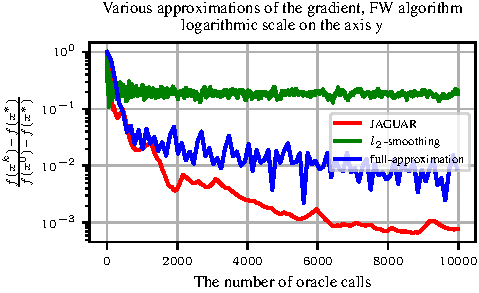
\includegraphics[width = 0.9\textwidth]{BachelorThesis_slides/pictures/Non_stochastics_FW_LogReg_Simplex.pdf}
    \end{figure}

\end{frame}

%----------------------------------------------------------------------------------------------------------

\begin{frame}{Эксперимент}

    Эксперимент проводился на симплексном множестве на квадратичной задаче.

    \begin{figure}
        \centering
        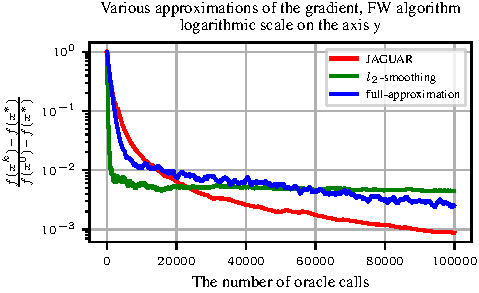
\includegraphics[width = 0.9\textwidth]{BachelorThesis_slides/pictures/Non_stochastics_FW_Reg_Simplex.pdf}
    \end{figure}

\end{frame}

%----------------------------------------------------------------------------------------------------------

\begin{frame}{Франк-Вульф с JAGUAR в стохастическом случае}

    Схемы аппроксимации:

    \begin{itemize}
        \item Двухточечная обратная связь:
            \begin{equation*}
                \widetilde{\nabla}_if_\delta(x, \xi) :=  \dfrac{f_\delta(x + \gamma e_i, \xi) - f_\delta(x - \gamma e_i, \xi)}{2 \gamma} e_i,
            \end{equation*}
        \item Одноточечная обратная связь:
            \begin{equation*}
                \widetilde{\nabla}_if_\delta(x, \xi^+, \xi^-) :=  \dfrac{f_\delta(x + \gamma e_i, \xi^+) - f_\delta(x - \gamma e_i, \xi^-)}{2 \gamma} e_i,
            \end{equation*}
    \end{itemize}

    где $e_i$ -- $i$-ый базисный вектор, $\gamma$ -- параметр сглаживания.

\end{frame}

%----------------------------------------------------------------------------------------------------------

\begin{frame}{Франк-Вульф с JAGUAR в стохастическом случае}

    \begin{algorithm}[H]
        \caption{ФВ с JAGUAR в стохастическом случае}
        \begin{algorithmic}[1]
        \State {\bf Вход:} $x^0 \in Q$, $h^0 = g^0 = \widetilde\nabla f_{\delta}(x^0, \xi_{\overline{1, d}}^\pm)$, $\gamma_k$, $\eta_k$, $\tau$
        \For {$k = 0, 1, 2, ... , N$}
            \State Сэмплируем $i \in \overline{1, d}$ независимо и равномерно
            \State Сэмплируем 2 реализации $\xi$: $\xi^+_k$ и $\xi^-_k$ независимо (в ДОС $\xi_k^+= \xi_k^-$)
            \State Считаем $\widetilde{\nabla}_{i_k} f_{\delta}(x^k, \xi^+_k, \xi^-_k) = \frac{f_{\delta}(x^k + \tau e_{i_k}, \xi^+_k) - f_{\delta}(x^k - \tau e_{i_k}, \xi^-_k)}{2 \tau} e_{i_k}$
            \State $h^{k+1} = h^k - \langle h^k, e_{i_k} \rangle e_{i_k} + \widetilde{\nabla}_{i_k} f_{\delta}(x^k, \xi^+_k, \xi^-_k)$
            \State $\rho^{k} = h^{k} - d \cdot \langle h^{k}, e_{i_k} \rangle e_{i_k} + d \cdot \widetilde{\nabla}_{i_k} f_{\delta}(x^k, \xi^+_k, \xi^-_k)$
            \State $g^{k+1} = (1 - \eta_k) g^k + \eta_k \rho^k$
            \State $s^k = \underset{s \in Q}{\arg\min}\left<s, g^{k+1} \right>$
            \State $x^{k+1} = x^k + \gamma_k (s^k - x^k)$
        \EndFor
        \State \textbf{Выход:} $x^{N + 1}$
        \end{algorithmic}
   \end{algorithm}
  
\end{frame}

%----------------------------------------------------------------------------------------------------------

\begin{frame}{Франк-Вульф с JAGUAR в стохастическом случае}

    Допущения:
    \small{
        \begin{enumerate}
            \item Функция $f(x, \xi)$ $L(\xi)$-гладкая на множестве $Q$: 
                \begin{equation*}
                    \forall x, y \in Q \hookrightarrow \left\|\nabla f(x, \xi) - \nabla f(y, \xi)\right\| \leq L(\xi) \left\|x-y\right\|.
                \end{equation*}

            \item Функция $f(x, \xi)$ выпукла на множестве $Q$:
                \begin{equation*}
                    \forall x, y \in Q: f(y, \xi) \geq f(x, \xi) + \langle \nabla f(x, \xi), y - x \rangle.
                \end{equation*}

            \item Ограниченность оракульного шума:
                \begin{equation*}
                    \exists \Delta > 0 : ~\forall x \in Q \hookrightarrow \expect{|\delta(x, \xi)|^2} \leq \Delta^2
                \end{equation*}

            \item Ограниченность второго момента градиента:
                \begin{equation*}
                    \exists \sigma^2_{\nabla} : \expect{\norms{\nabla f(x, \xi) - \nabla f(x)}^2} \leq \sigma^2_{\nabla}
                \end{equation*}

            \item Ограниченность второго момента оракула (для ООС):
                \begin{equation*}
                    \exists \sigma^2_{f} : \expect{\left|f(x, \xi) - f(x) \right|^2} \leq \sigma^2_{f}
                \end{equation*}
            
        \end{enumerate}
        }

\end{frame}

%----------------------------------------------------------------------------------------------------------

% \begin{frame}{Франк-Вульф с JAGUAR в стохастическом случае}
    
%     \begin{algorithm}[H]
%         \caption{ФВ с JAGUAR в стохастическом случае}
%         \begin{algorithmic}[1]
%                 \State {\bf Вход:} $x_0 \in Q$, $h^0 = g^0 = \widetilde\nabla f_{\delta}(x^0, \xi_1^+, ...., \xi_d^-)$, $\{\eta_k\}_{k=0}^N \subset [0; 1]$
                
%         	    \For {k = 0, 1, 2, ... , N}
%                     \State $h^{k+1}, g^{k+1} = $ JAGUAR $\left( x^k, h^k, g^k, \eta_k \right)$
                    
%                     \State $s^k = \underset{x \in Q}{\arg\min}\left\{\left<s, g^{k+1} \right> \right\}$
                    
%                     \State $x^{k+1} = x^k + \gamma_k (s^k - x^k)$ \label{line:x^k}
%                 \EndFor
%             \State \textbf{Выход:} $x^{N+1}$ 
%         	\end{algorithmic}
%         \end{algorithm}
        
% \end{frame}

%----------------------------------------------------------------------------------------------------------

% \begin{frame}{JAGUAR. Стохастический случай}

%     \textbf{Теорема} При шаге оптимизатора и шаге моментума:
            
%         $$\gamma_k = \frac{4}{k + 8d^{3/2}}, \quad \eta_k = \frac{4}{(k + 8d^{3/2})^{2/3}}$$
            
%         получается следующее:

%         \small{
%             \begin{equation*}
%                 \begin{split}
%                     \expect{\norms{g^k - \nabla f(x^k)}^2} 
%                     &=
%                     \mathcal{O} \Bigg( \frac{d^4 \norms{h^0 - \nabla f(x^0)}^2}{(k + 8d^{3/2})^{8/3}} + d L^2 \gamma^2 + \frac{d \Delta^2}{\gamma^2}
%                     \\&+
%                     \frac{L^2 D^2 + \max\{d^2 \sigma_f^2/ \gamma^2 + d^2 \sigma_{\nabla}^2, d \norms{g^0 - \nabla f(x^0)}^2\}}{(k + 8d^{3/2})^{2/3}}  
%                     \Bigg)
%                 \end{split} 
%             \end{equation*}
%         }

%         Если $h^0 = g^0 = \widetilde{\nabla} f_\delta(x^0, \xi^+_1, \xi^-_1, ..., \xi^+_d, \xi^-_d)$, то можно упростить:
    
%         \begin{equation*}
%             \expect{\norms{g^k - \nabla f(x^k)}^2} = \mathcal{O} \left(\frac{L^2 D^2 + d^2 \sigma_f^2/ \gamma^2 + d^2 \sigma_{\nabla}^2}{(k + 8d^{3/2})^{2/3}} + d L^2 \gamma^2 + \frac{d \Delta^2}{\gamma^2} \right)
%         \end{equation*}
            
% \end{frame}

%----------------------------------------------------------------------------------------------------------

\begin{frame}{Франк-Вульф с JAGUAR в стохастическом случае}

    \textbf{Теорема} При шаге оптимизатора и шаге моментума:
        \begin{equation*}
            \gamma_k = \frac{4}{k + 8d^{3/2}}, \quad \eta_k = \frac{4}{(k + 8d^{3/2})^{2/3}}
        \end{equation*}
            
        получается оценка на сходимость:
        \small{
             \begin{align*}
                    \mathbb{E}\left[f(x^{N}) - f(x^*) \right] = \mathcal{O}
                    &\Bigg(
                    \frac{L D^2 + d \sigma_f D/ \gamma + d \sigma_{\nabla} D + \sqrt{d} (f(x^0) - f(x^*))}{(N + 8d^{3/2})^{1/3}} \\
                    &+
                    \sqrt{d} L D \gamma + \frac{\sqrt{d} \Delta D}{\gamma} \Bigg)
             \end{align*}
        }

        \textbf{Следствие} Пусть $\varepsilon$ определяет точность: $\expect{f(x^N) - f(x^*)} \leq \varepsilon$:

        \begin{equation*}
            N = \mathcal{O} \left( \max\left\{ \left[ \frac{L D^2 + d\sigma_{\nabla} D + \sqrt{d} (f(x^0) - f(x^*))}{\varepsilon}\right]^3 , \frac{d^{9/2} \sigma_f^3 L^3D^6}{\varepsilon^6} \right\}\right),
        \end{equation*}
        
        \begin{equation*}
            \gamma = \mathcal{O} \left(\frac{\varepsilon}{\sqrt{d} L D} \right), \quad
            \Delta = \mathcal{O} \left( \frac{\varepsilon^2}{d L D^2}\right).
        \end{equation*}
            
\end{frame}

%----------------------------------------------------------------------------------------------------------

\begin{frame}{Эксперимент}

    Эксперимент проводился на $L2$-шаре на квадратичной задаче.

    \begin{figure}
        \centering
        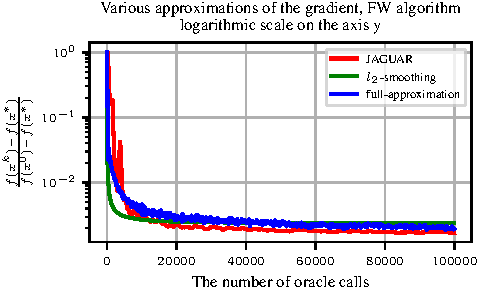
\includegraphics[width = 0.9\textwidth]{BachelorThesis_slides/pictures/Stochastics_TPF_FW_Reg_L2.pdf}
    \end{figure}

\end{frame}

%----------------------------------------------------------------------------------------------------------

\begin{frame}{Эксперимент}

    Эксперимент проводился на симплексном множестве на квадратичной задаче.

    \begin{figure}
        \centering
        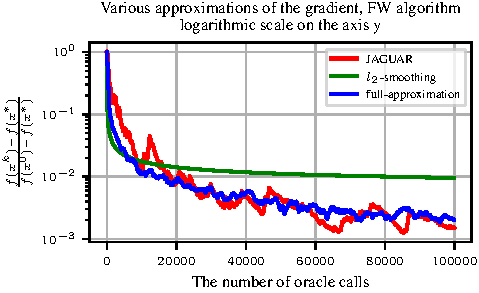
\includegraphics[width = 0.9\textwidth]{BachelorThesis_slides/pictures/Stochastics_TPF_FW_Reg_Simplex.pdf}
    \end{figure}

\end{frame}

%----------------------------------------------------------------------------------------------------------

\begin{frame}{Вывод}

    Для выпуклой задачи оптимизации на ограниченном выпуклом множестве с доступом только к нулевому оракулу предложена и исследована модификация JAGUAR для алгоритма Франка-Вульфа. Получены теоретические оценки сходимости для нестохастического и стохастического случаев. Поставлены эксперименты на различных задачах и различных множествах.
    
\end{frame}

%----------------------------------------------------------------------------------------------------------

% \begin{frame}{Дальнейшая работа}

%     \begin{itemize}
%         \item Исправить метрику на $gap$, которой обычно измеряют сходимость алгоритма Франка-Вульфа;
%         \item Возможно, рассмотреть другие методы, например, градиентный спуск;
%         \item Рассмотреть ускоренные методы.
%     \end{itemize}

% \end{frame}

%----------------------------------------------------------------------------------------------------------

% \begin{frame}{Эксперимент}

%     Эксперимент проводился на симплексном множестве на квадратичной задаче.

%     \begin{figure}
%         \centering
%         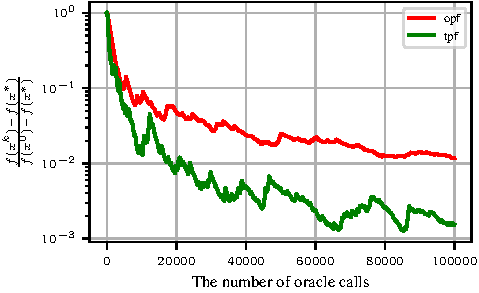
\includegraphics[width = 0.9\textwidth]{BachelorThesis_slides/figures/Stochastics_OPF_TPF_FW_Reg_Simplex.pdf}
%     \end{figure}

% \end{frame}

%----------------------------------------------------------------------------------------------------------

\end{document}